\newpage
\section{UI structure}

\subsection{Bill}
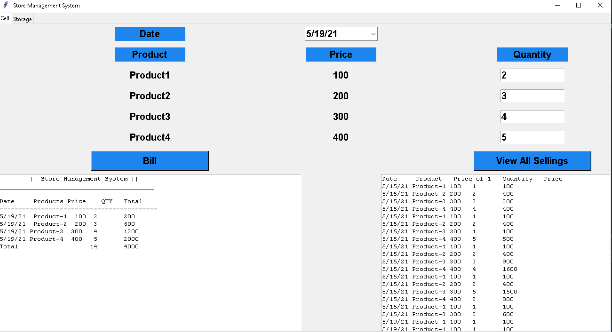
\includegraphics{images/Demo1 Bill.png}


\hspace{0.7cm}
In those blanks, it helps staff manage bills.
When you enter information in the corresponding boxes and press the bill button, the system will show that customer's invoice in the lower left corner table. When you click the viewallsselling button, the system will show the sales history.


   \item Quantity: Users only need to enter the purchase quantity of that customer in the blank box corresponding to the product name next to it.
   \item Bill: It shows the quantity, product name, and price of that product. What the customer bought along with the total amount to be paid and the time it took for the transaction to take place.
   \item ViewAllSelling: The system will give the store's transaction history along with the transaction date.
   
\newpage
\subsection{Storage}
\vspace{1cm}
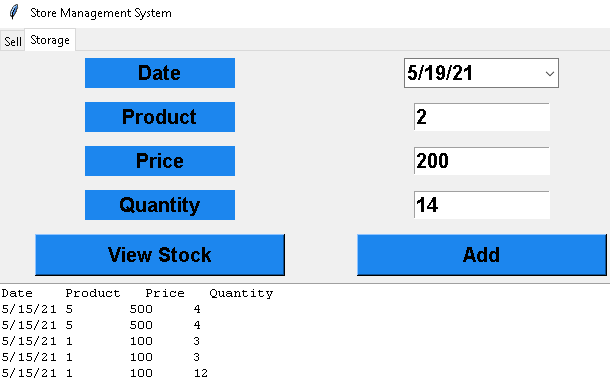
\includegraphics{images/Demo2 Stock.png}



\vspace{1cm}
\textbf{It is a user interface structure that helps users manage inventory, import and export goods.}
\begin{itemize}
    \item Add : the user enters the information of the new product in each of the same blank boxes.
    \item View Stock: The system will show information of the products that the user has entered.
 
\end{itemize}

